\documentclass{ufpatcc}
\usepackage{lipsum}
\begin{document}
% FRONT MATTER -------------------------------------------%
  \capa
  \folhaderosto
  \pagenumbering{arabic}
  \fichacatalografica{Biblioteca Prof. Dr. Clodoaldo Beckmann}
                     {1. Área 2. Outra área I. Título.}
                     {21.ed. 001.1}
  \folhadeaprovacao{17/06/2018}
  \begin{dedicatoria}
    \lipsum[13]
  \end{dedicatoria}
  \begin{agradecimentos}
    \lipsum[1-5]
  \end{agradecimentos}
  \begin{epigrafe}
    ``\lipsum*[101]''\par
      Autor
  \end{epigrafe}
  \begin{resumo}
    \lipsum[1]
  \end{resumo}
  \begin{abstract}
    \lipsum[1]
  \end{abstract}
  \tableofcontents

	% --------------------- 
	%	INICIO DOS CAPÍTULOS	
	% --------------------- 
	
	% --------------------- 
	%	INTRODUÇÃO 	
	% --------------------- 
  \chapter{Introdução} % ou \input{arquivoexterno}
		
		Contextualização; Estado da arte (se tiver); Motivação; O que vai fazer; Metodologia; O que terá no resto do documento;


	% --------------------- 
	%	REFERENCIAL TEÓRICO	
	% --------------------- 
	\chapter{Referencial Teórico}

		\section{Sensor Flex}
		Sensores de flexão, mais conhecidos como sensores flex, são resistores analógicos que trabalham como divisores de tensão analógicos. Dentro desses sensores existem elementos resistivos de carbono junto a um fino substrato flexível. Mais carbono significa menos resistência. Quando o substrato é torcido o sensor produz uma resistência relativa ao raio da torção. \cite{solanki2013sign}

		\begin{figure}[h!]
  		\label{fig:flex-sensor1}
			\centering
  		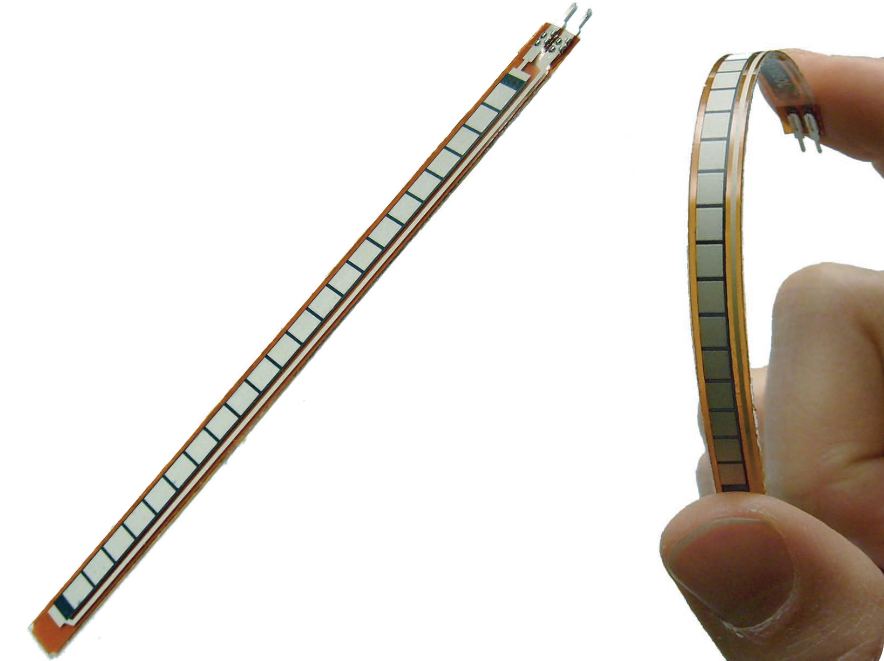
\includegraphics[scale=0.4]{../pictures/flex-sensor-sparkfun.png}
  		\caption{Sensor Flex}
		\end{figure}


		\section{Potenciômetro}
		O potenciômetro é um componente eletrônico que permite, através do giro do seu eixo, a variação da resistência entre seus terminais. Eles são constituídos por um elemento de resistência, que pode ser de carbono ou fio de nicromo, sobre o qual corre uma lingüeta, denominada cursor. Dentre as características do potenciômetro estão o valor máximo de sua resistência, seu número de voltas, seu grau máximo de giro (aproximado) e se ele é do tipo linear ou logarítmico \cite{ncb2012eletronicabasica}.


		\begin{figure}[h!]
  		\label{fig:pot1}
			\centering
  		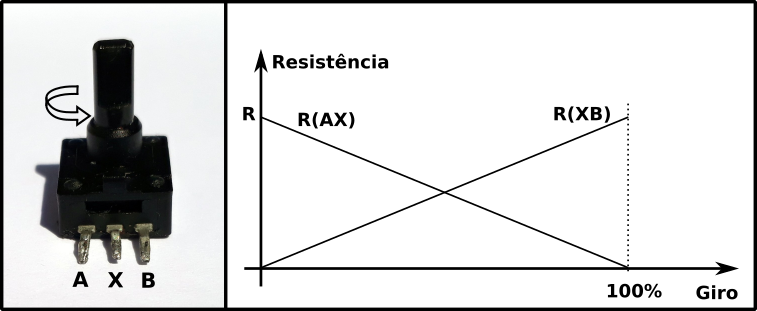
\includegraphics[scale=0.7]{../pictures/potentiometer1.png}
  		\caption{Funcionamento do potenciômetro linear}
		\end{figure}

		Segundo a lei de Ohm ($V = R.I$), dada uma corrente constante, ao variar a resistência teremos uma variação da tensão. Sendo assim, ao girar o eixo do potenciômetro, dependendo do sentido do giro, perceberemos um aumento ou diminuição da tensão naquele ponto. Partindo de um ponto extremo com resistência mínima até o outro ponto extremo no qual a resistência deverá ser a máxima característica do componente.

		\section{Movimentação dos dedos}
		Na mão, os tendões funcionam como cordas que conectam os músculos do antebraço aos ossos da mão. Nos dedos, os tendões passam por dentro de uma série de polias, que formam uma espécie de túnel. Isso permite manter os tendões próximos aos ossos da mão, aumentando a força nos dedos e diminuindo o gasto de energia. Ao movimentar o dedo, o músculo se contrai para que o tendão deslize por entre as polias. \cite{drricardocirurgiao}
 
		\begin{figure}[h!]
  		\label{fig:hand-move1}
			\centering
  		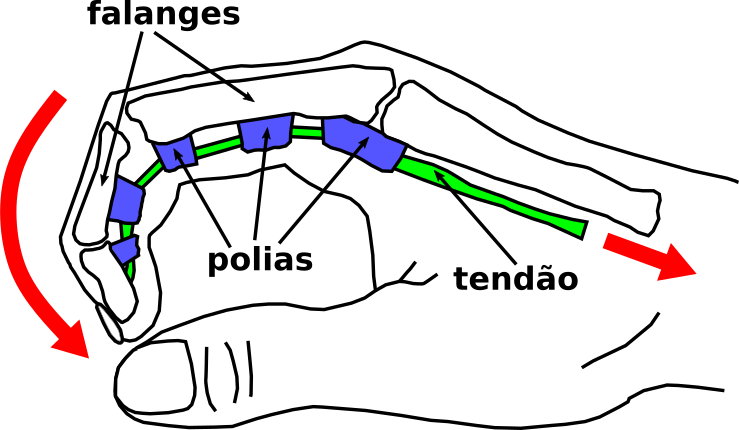
\includegraphics[scale=0.5]{../pictures/hand-flex-movement1.png}
  		\caption{Movimento do dedo através do tendão}
		\end{figure}

		\section{Arduino}
		O Arduino é uma plataforma eletrônica de código aberto (\textit{open-source}) que é baseada em \textit{hardware} e \textit{software} fáceis de usar. As placas Arduino são capazes de ler entradas como o acionamento de um sensor, o pressionamento de um botão, ou uma mensagem do Twitter. E pode transformar essas entradas em saídas como a ativação de um motor, o acendimento de um LED ou até a publicação de algo online. O comportamento dessa placa pode ser programado usando sua interface de desenvolvimento (IDE), que por sua vez, envia as instruções necessárias para o microcontrolador instalado na placa.\cite{arduinosite}
		
		\begin{figure}[h!]
  		\label{fig:arduino-nano1}
			\centering
  		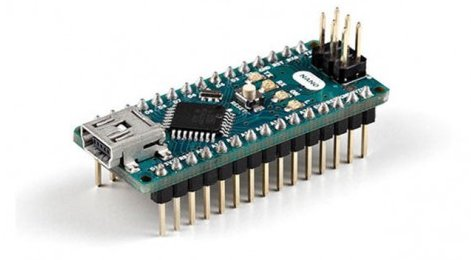
\includegraphics[scale=0.7]{../pictures/arduino-nano1.jpg}
			\caption{Placa Arduino modelo Nano \cite{arduinonanosite}}
		\end{figure}

		\section{Módulo RF 433 Mhz}
		O módulo de rádio frequência 433 Mhz é composto por um par que contém um transmissor e um receptor, ele opera com modulação AM e é uma alternativa para projetos de baixo custo que queiram usar comunicação sem fio entre microcontroladores Arduino ou outros. O par de módulos pode alcançar até 200 metros sem obstáculos, usando antenas e dependendo da tensão aplicada.\cite{institutodigitalrf}
		
		



	% ----------------------------
	%	TRABALHO PROPRIAMENTE DITO	
	% ----------------------------
	\chapter{Trabalho Propriamente Dito}

		\section{Teoria da coisa}
			Como foi demonstrado na figura \ref{fig:hand-move1}, através dos tendões, passando por polias, têm-se a movimentação dos dedos na mão. Baseado nessa biomecânica de movimento, foi desenvolvido um sistema mecânico semelhante, com o intuito de criar um sensor de flexão de dedos, atrelado a um transmissor de dados.
			
			Inicialmente foi verificado o deslocamento de um fio durante a flexão dos dedos. Para isso, com a mão inicialmente extendida e o dorso voltado para cima, uma das pontas de um fio foi presa na ponta de um dos dedos. O local inicial da outra ponta do fio foi marcada no dorso mão.

			Após a flexão dos dedos o fio se movimentou em uma direção criando um deslocamento (d) do fio em relação ao ponto marcado.


		\begin{figure}[h!]
  		\label{fig:hand-flex1}
			\centering
  		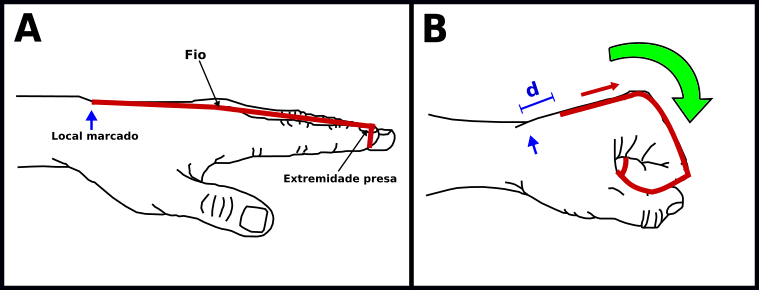
\includegraphics[scale=0.7]{../pictures/hand-flex1.png}
			\caption{Mão em posição inicial (A) e após a flexão dos dedos (B)}
		\end{figure}


			Após examinar esse movimento, foi decidido criar e instalar todo o sistema em uma luva. Fios foram presos às extremidades dos dedos da luva, passando por polias plásticas que servem de guias. Na extremidade oposta, os fios são conectados à pequenos potenciômetros que variam de acordo com o sentido do movimento de cada fio. Sendo assim, para os cinco dedos de cada mão, são utilizados cinco fios e cinco potenciômetros.

			A variação de cada potenciômetro é captada por um microcontrolador que processa esse sinal antes de despachá-lo para o transmissor. O módulo transmissor envia por rádio frequência, mensagens em formato de números inteiros que representam a posição atual de cada dedo.

		\begin{figure}[h!]
  		\label{fig:glove-and-transmitter1}
			\centering
  		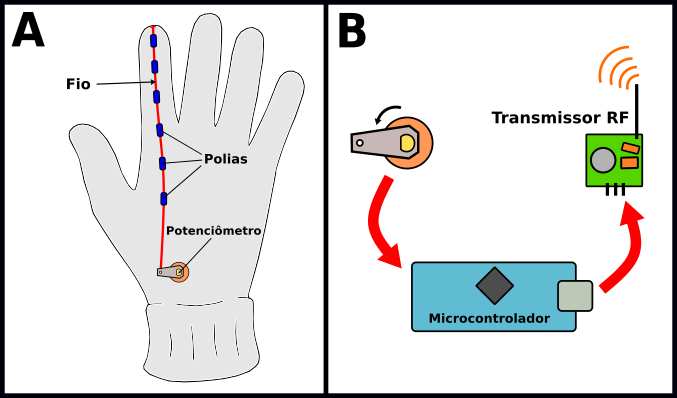
\includegraphics[scale=0.7]{../pictures/glove-and-transmitter1.png}
			\caption{Captação (A) e transmissão do sinal (B)}
		\end{figure}

			O módulo receptor de rádio frequência, capta as mensagens e as envia ao microcontrolador conectado. Este por sua vez, processa a mensagem e transmite aos respectivos componentes e atuadores daquela aplicação.

			Para este trabalho, um pequeno carrinho, foi o sistema escolhido para ser controlado pela luva. Para isso, um protocolo de transmissão foi desenvolvido para traduzir os movimentos dos dedos da luva em direções para o carrinho.
	
		\begin{figure}[h!]
  		\label{fig:receptor-to-app1}
			\centering
  		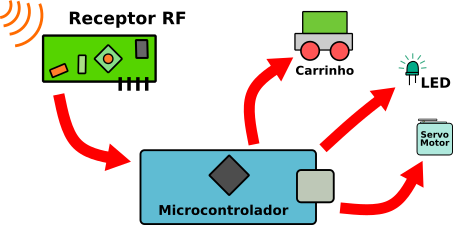
\includegraphics[scale=0.8]{../pictures/receptor-to-app1.png}
			\caption{Recepção e processamento do sinal}
		\end{figure}
		\section{Medidas e Posicionamento}	

		\section{Placa de Circuito Impresso}
		
		\section{Movimento mecânico}


	% ----------------------------
	%	RESULTADOS E ANÁLISES	
	% ----------------------------
	\chapter{Análises e Resultados}

		\section{Configurações}

		\section{Testes}

		\section{Resultados}
		

	% ----------
	%	CONCLUSÃO	
	% ----------
  \chapter{Conclusão}

		\section{Conclusões}

		\section{Trabalhos Futuros}

	% ----------------------------
	%	REVISÃO BIBLIOGRÁFICA	
	% ----------------------------
  \chapter{Revisão Bibliográfica}
%    \lipsum[1]\cite{atalholivro}
    \lipsum[2]\cite{atalhoonline}


% BACK MATTER --------------------------------------------%
  \appendix
    \chapter{Algum apêndice}
    \chapter{Outro apêndice}

  \bibliographystyle{IEEEtran}
  \referencias{referencias}
\end{document}
